\documentclass{article}
\usepackage{tikz}
\usetikzlibrary{external,shapes,calc,math,patterns,arrows,positioning,fadings}
\tikzexternalize[optimize=false]

\tikzstyle{node}=[circle, draw=black, fill=white, minimum size=20pt, line width=1, inner sep= 2pt]
\tikzstyle{nodel}=[circle, draw=black, fill=white, minimum size=5pt, line width=1, inner sep= 0pt]
\tikzstyle{node2}=[circle, draw=black, fill=white, minimum size=8pt, line width=1, inner sep= 0pt, fill=white!70!black]
\tikzstyle{l1}=[line width=1]
\tikzfading[name=fade right, left color=transparent!0, right color=transparent!100]

\begin{document}
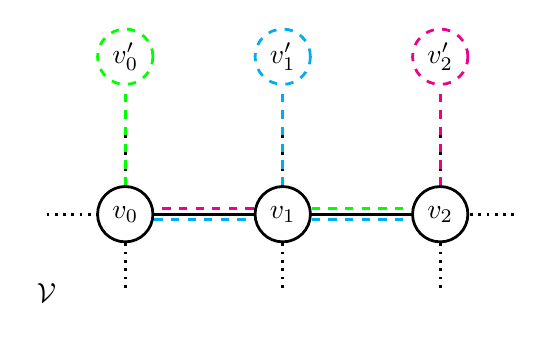
\begin{tikzpicture}[scale=1]
    \node at (-1, -1) {$\mathcal{V}$};
    \draw[l1] (0, 0) -- (4,0);
    \draw[l1, dotted] (-1,0) -- (5,0);
    \draw[l1, dotted] (0,1) -- (0,-1);
    \draw[l1, dotted] (2,1) -- (2,-1);
    \draw[l1, dotted] (4,1) -- (4,-1);
    \node[node] at (0,0) (1) {$v_0$};
    \node[node, draw=green, dashed] at (0,2) (2) {$v_0'$};
    \node[node] at (2,0) (3){$v_1$};
    \node[node, draw=cyan, dashed] at (2,2) (4) {$v_1'$};
    \node[node] at (4,0) (5) {$v_2$};
    \node[node, draw=magenta, dashed] at (4,2) (6) {$v_2'$};

    \draw[l1, dashed, green] (1) -- (2);
    \draw[l1, dashed, green, transform canvas={yshift=2pt}] (3) -- (5);
    \draw[l1, dashed, cyan] (3) -- (4);
    \draw[l1, dashed, cyan, transform canvas={yshift=-2pt}] (1) -- (3) -- (5);
    \draw[l1, dashed, magenta] (5) -- (6);
    \draw[l1, dashed, magenta, transform canvas={yshift=2pt}] (3) -- (1);
\end{tikzpicture}

\begin{tikzpicture}[scale=0.6]
    \node[node, fill=white!70!green] at (0,0) (0) {$\sigma_0$};
    \node[node, fill=white!70!cyan] at (2,0) (1) {$\sigma_1$};
    \node[node, fill=white!70!black, path fading=fade right] at (4,0) (5) {$\sigma_2$};
    \node[node] at (-2,0) (2) {$v_3$};
    \node[node] at (0,2) (3) {$v_4$};
    \node[node] at (0,-2) (4) {$v_5$};
    \draw[l1] (1) -- (0) -- (3);
    \draw[l1] (2) -- (0) -- (4);
    \draw[l1, dotted] (2, 1.5) -- (1) -- (2,-1.5);
    \draw[l1] (1) -- (5);
    \fill[color=green!50!white, opacity=0.3] (0,3) arc (90:225:1) arc (45:-135:.4142) arc (45:315:1) arc (135:-45:.4142) arc (135:405:1) arc (225:135:.4142) arc (-45:45:1) arc (225:135:.4142) arc (-45:90:1) -- cycle;
    \fill[color=cyan!50!white, opacity=0.3] (2,1) arc (90:450:1);

    \node at (-2, 2.5) {$\mathcal{V}$};
    \node at (2, -2.5) {$\mathcal{N}:$};

    \node[nodel, fill=white!70!green] at (2.8, -2.55) (d) {};
    \node[nodel, fill=white!70!cyan] at (3.3, -2.55) (e) {};
    \node[nodel, fill=white!70!black] at (3.8, -2.55) (f) {};
    \draw[l1] (d) -- (e) -- (f);
\end{tikzpicture}

\end{document}